\documentclass[12pt,titlepage]{article}
\usepackage[margin=1.25in]{geometry}
\usepackage{graphicx,amsmath,blindtext}

%% Variables definition
\newcommand{\vSubject}{@Subject}
\newcommand{\vSubtitle}{@Subtitle}
\newcommand{\vName}{@Name}
\newcommand{\vNIM}{@NIM}
\newcommand{\vClass}{@Class}
\newcommand{\vDepartment}{@Department}
\newcommand{\vStudyProgram}{@StudyProgram}

%% [START] Tikz related stuff
\usepackage{tikz}
\usetikzlibrary{svg.path,calc,shapes.geometric,shapes.misc}
\tikzstyle{terminator} = [rectangle, draw, text centered, rounded corners = 1em, minimum height=2em]
\tikzstyle{preparation} = [chamfered rectangle, chamfered rectangle sep=0.75em, draw, text centered, minimum height = 2em]
\tikzstyle{process} = [rectangle, draw, text centered, minimum height=2em]
\tikzstyle{decision} = [diamond, aspect=2, draw, text centered, minimum height=2em]
\tikzstyle{data}=[trapezium, draw, text centered, trapezium left angle=60, trapezium right angle=120, minimum height=2em]
\tikzstyle{connector} = [line width=0.25mm,->]
%% [END] Tikz related stuff

%% [START] Fancy header related stuff
\usepackage{fancyhdr}
\pagestyle{fancy}
\setlength{\headheight}{15pt} % compensate fancyhdr style
\fancyhead{}
\fancyfoot{}
\fancyfoot[L]{\thepage}
\fancyfoot[R]{\textit{\vSubject - \vSubtitle}}
\renewcommand{\footrulewidth}{0.4pt}% default is 0pt, overline for footer
%% [END] Fancy header related stuff

%% [START] Custom tabular command related stuff
\usepackage{tabularx}
\newcommand{\details}[2]{
    #1 & #2  \\
}
%% [END] Custom tabular command related stuff

%% [START] Figure related stuff
\newcommand{\image}[3][1]{
    \begin{figure}[h]
        \centering
        \includegraphics[#1]{#2}
        \caption{#3}
        \label{#3}
    \end{figure}
}
%% [END] Figure related stuff

\begin{document}
\begin{titlepage}
    \centering
    \vfill
    {\bfseries\LARGE
        \vSubject\\
        \vskip0.25cm
        \vSubtitle
    }
    \vfill
    
\includegraphics[width=6cm]{images/polinema-logo.png}
    \vfill
    {
        \textbf{Name}\\
        \vName\\
        \vskip0.5cm
        \textbf{NIM}\\
        \vNIM\\
        \vskip0.5cm
        \textbf{Class}\\
        \vClass\\
        \vskip0.5cm
        \textbf{Department}\\
        \vDepartment\\
        \vskip0.5cm
        \textbf{Study Program}\\
        \vStudyProgram
    }
\end{titlepage}

\section{Section One - \LaTeX}
\subsection{Experiment 1: This is an example of list items}
\textbf{Questions}
\begin{enumerate}
    \item {
        Some questions could go here...!

        \begin{itemize}
            \item Item number one
            \item Another item
            \item Some \textbf{BOLD} item
        \end{itemize}
    }
    \item {
        Maybe another question?

        \begin{itemize}
            \item Another list?
            \item \textit{No?}
        \end{itemize}
    }
    \item {
        A template for doing left-right colon alignment

        \begin{tabularx}{\textwidth}[t]{@{}>{\bfseries}l!{:}X}
        \details{Input}{Could be anything}
        \details{Output}{Something}
        \details{Other Data}{-}
        \details{Process}{
            \begin{itemize}
                \item Item number one, again
                \item Love me some math. $$f(x) = ax^2 + bx + c$$
            \end{itemize}
        }
        \end{tabularx}
    }
    \pagebreak
    \item {
        Example of using image with caption and stuff

        \image[width=4cm]{images/polinema-logo.png}{Polinema Logo}

        \blindtext
    }
    \item {
        Use tikz to draw some graph or some sort of flowchart

        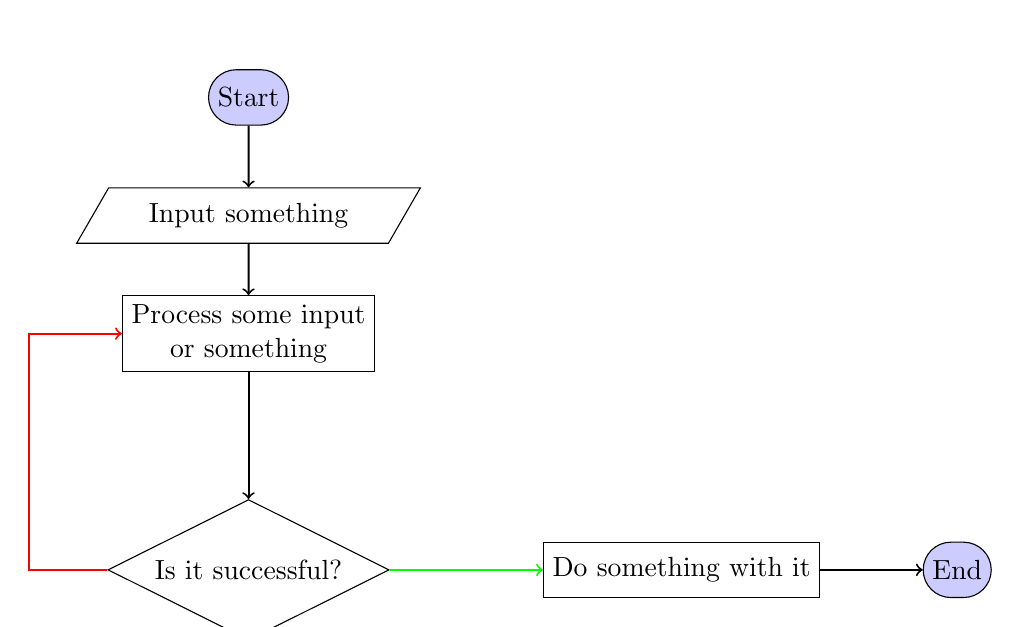
\begin{tikzpicture}[node distance = 1.5cm]
            \node (start) [terminator,fill=blue!20] {Start};
            \node (data) [data,below of = start] {Input something};
            \node (process) [process,below of = data,align=center] {Process some input\\or something};
            \node (branch) [decision,below of = process,yshift=-1.5cm] {Is it successful?};
            \node (process2) [process,right of = branch,xshift=4cm] {Do something with it};
            \node (end) [terminator, right of = process2,xshift=2cm,fill=blue!20] {End};
            \draw [connector] (start) -- (data);
            \draw [connector] (data) -- (process);
            \draw [connector] (process) -- (branch);
            \draw [connector,green] (branch) -- (process2);
            \draw [connector,red] (branch.west) -- ($(branch.west)+(-1cm,0)$) |- (process.west);
            \draw [connector] (process2) -- (end);
        \end{tikzpicture}
    }
\end{enumerate}

\end{document}

